\documentclass[12pt]{article}

% ===== Configuración común =====
\newcommand{\commonpath}{../../common}
% ===== Idioma y codificación =====
\usepackage[spanish, es-nodecimaldot]{babel}
\usepackage[utf8]{inputenc}
\usepackage[T1]{fontenc}
\usepackage{textcomp}

% ===== Tipografía moderna =====
\usepackage{helvet}
\renewcommand{\familydefault}{\sfdefault}
\usepackage{microtype}
\usepackage{xcolor}

% ===== Márgenes y formato =====
\usepackage[a4paper,top=2.8cm,bottom=2.8cm,left=3cm,right=3cm]{geometry}
\usepackage{titlesec}
\titleformat{\section}{\Large\bfseries}{\thesection.\ }{0.4em}{}
\titleformat{\subsection}{\large\bfseries}{\thesubsection.\ }{0.4em}{}
\titlespacing*{\section}{0pt}{1.6ex plus .5ex minus .2ex}{1.0ex}
\titlespacing*{\subsection}{0pt}{1.2ex plus .5ex minus .2ex}{0.7ex}

% ===== Colores =====
\definecolor{UMABlue}{RGB}{0,51,102}

% ===== Paquetes útiles =====
\usepackage{amsmath}
\usepackage{amssymb}
\usepackage{graphicx}
\usepackage{booktabs}
\usepackage{tabularx}
\usepackage{siunitx}
\usepackage{float}
\usepackage{enumitem}
\usepackage{listings}
\usepackage[hidelinks]{hyperref}
\usepackage{tikz}
\usetikzlibrary{arrows.meta, decorations.markings, patterns}
\sisetup{locale=DE}

% ===== Estilo para listados de código =====
\lstset{
  language=C++,
  basicstyle=\ttfamily\footnotesize,
  keywordstyle=\bfseries\color{UMABlue},
  commentstyle=\itshape\color{gray},
  stringstyle=\color{red!60!black},
  numbers=left,
  numberstyle=\tiny\color{gray},
  numbersep=6pt,
  frame=single,
  framerule=0.4pt,
  rulecolor=\color{gray!50},
  breaklines=true,
  tabsize=4,
  showstringspaces=false,
  captionpos=b,
  aboveskip=8pt,
  belowskip=6pt,
}

% ===== Comandos personalizados — Ampliación de Robótica =====

% --- Abreviaturas frecuentes ---
\newcommand{\ros}{ROS~2}
\newcommand{\roshumble}{ROS~2 Humble}
\newcommand{\coppelia}{CoppeliaSim}
\newcommand{\pioneer}{Pioneer P3DX}

% --- Unidades ---
\newcommand{\ms}{\si{\meter\per\second}}
\newcommand{\hz}[1]{\SI{#1}{\hertz}}
\newcommand{\rad}{\si{\radian}}

% --- Pendiente (texto rojo para secciones por completar) ---
\newcommand{\pendiente}[1]{\textcolor{red}{\textbf{[PENDIENTE:} #1\textbf{]}}}

% ===== Portada reutilizable =====
% Uso: \portada{LAB-ID}{Título}{Subtítulo}
\newcommand{\portada}[3]{%
  {%
    \pagecolor{UMABlue}%
    \color{white}%
    \thispagestyle{empty}%
    \begin{center}
      \vspace*{0.8cm}
      
\includegraphics[width=0.22\textwidth]{\commonpath/img/logo_uma.png}\\[0.5cm]
      {\large UNIVERSIDAD DE MÁLAGA\\[0.3cm]}
      {\small Grado en Ingeniería Electrónica, Robótica y Mecatrónica\\[1.2cm]}
      {\huge\bfseries Memoria de Práctica\\[0.6cm]}
      {\LARGE\bfseries #1\\[0.2cm]}
      {\Large\bfseries #2\\[0.4cm]}
      {\normalsize\itshape #3\\[1.8cm]}
      {\normalsize Ampliación de Robótica\\[0.8cm]}
      {\large
        Saúl Gutiérrez Rodríguez\\[0.15cm]
        Pablo Haro García\\[0.15cm]
        Mario Merino Prado\\[0.8cm]
      }
      \rule{0.55\textwidth}{0.4pt}\\[0.3cm]
      {\small
        Repositorio: \texttt{github.com/marioomerino24/ampliacion\_robotica}\\[0.1cm]
        Entorno: \roshumble{} · \coppelia{} · \pioneer{}
      }
    \end{center}
    \clearpage
  }%
  \nopagecolor%
  \color{black}%
}

\graphicspath{{figures/}{\commonpath/img/}}

% ===== Documento =====
\begin{document}

\portada{Lab-MR2}{Percepci\'{o}n del entorno}%
        {Estimaci\'{o}n de paredes por m\'{i}nimos cuadrados y Pure Pursuit}

\tableofcontents
\clearpage


% =====================================================================
%  1. INTRODUCCIÓN
% =====================================================================
\section{Introducci\'{o}n}

\subsection{Objetivo de la pr\'{a}ctica}
El objetivo es mejorar el seguimiento de pasillo de la pr\'{a}ctica anterior sustituyendo las lecturas puntuales del l\'{a}ser por un \textbf{modelo geom\'{e}trico de las paredes} obtenido mediante regresi\'{o}n lineal por m\'{i}nimos cuadrados. En lugar de promediar rangos en ventanas angulares estrechas, se ajusta una recta $y = mx + b$ a cada pared, lo que proporciona simult\'{a}neamente la \textbf{distancia} (intercepto $b$) y la \textbf{orientaci\'{o}n} (pendiente $m$) del robot respecto a cada pared.

\subsection{Descripci\'{o}n del problema}
El robot \pioneer{} navega por un pasillo cerrado con un l\'{a}ser 2D. El problema consiste en:
\begin{enumerate}[leftmargin=2em]
  \item \textbf{Extraer} la ecuaci\'{o}n de cada pared (izquierda y derecha) a partir de la nube de puntos l\'{a}ser en coordenadas cartesianas.
  \item \textbf{Calcular} el centro del pasillo a una distancia de look-ahead $L$ usando los modelos de ambas paredes.
  \item \textbf{Aplicar} Pure Pursuit sobre ese punto objetivo para mantener el robot centrado.
\end{enumerate}

La ventaja respecto al enfoque de la pr\'{a}ctica anterior (Lab-MR1-II) es que el modelo de recta integra \textbf{todas las lecturas} de un sector angular amplio, lo que reduce el efecto del ruido y proporciona informaci\'{o}n de orientaci\'{o}n sin necesidad de heur\'{i}sticas adicionales.


% =====================================================================
%  2. FUNDAMENTOS TEÓRICOS
% =====================================================================
\section{Fundamentos te\'{o}ricos}

\subsection{Modelo cinem\'{a}tico del robot}
El \pioneer{} utiliza tracci\'{o}n diferencial con $R = \SI{0.097518}{\meter}$ y $2K = \SI{0.331}{\meter}$. Como en la pr\'{a}ctica anterior, se comanda directamente $(v, \omega)$ al simulador mediante el topic \texttt{cmd\_vel}.

\subsection{Algoritmo de control: Pure Pursuit con modelo de paredes}
El controlador utiliza \textbf{Pure Pursuit} (ecuaci\'{o}n~\eqref{eq:pure_pursuit}), pero en lugar de construir el punto objetivo a partir de distancias puntuales, lo calcula a partir de las rectas ajustadas a cada pared.

Si la pared izquierda se modela como $y = m_L x + b_L$ y la derecha como $y = m_R x + b_R$, la coordenada $y$ del centro del pasillo a una distancia $x = L$ (look-ahead) del robot es:
\begin{equation}
  y_\text{goal} = \frac{(m_L + m_R)}{2} \cdot L + \frac{b_L + b_R}{2}
  \label{eq:y_goal}
\end{equation}

La curvatura comandada es:
\begin{equation}
  \kappa = \frac{2\,y_\text{goal}}{L^2}
  \label{eq:pure_pursuit}
\end{equation}

y las velocidades:
\begin{equation}
  v = \frac{v_\text{max}}{2}, \qquad
  \omega = \text{clamp}(\kappa \cdot v,\; -\omega_\text{max},\; \omega_\text{max})
  \label{eq:velocidades}
\end{equation}

\subsection{Procesamiento sensorial: regresi\'{o}n lineal por m\'{i}nimos cuadrados}
Dado un conjunto de $n$ puntos l\'{a}ser $(x_i, y_i)$ pertenecientes a una pared, se busca la recta $y = mx + b$ que minimiza la suma de errores cuadr\'{a}ticos. La soluci\'{o}n anal\'{i}tica es:

\begin{equation}
  m = \frac{n \sum x_i y_i - \sum x_i \sum y_i}{n \sum x_i^2 - \left(\sum x_i\right)^2}, \qquad
  b = \frac{\sum y_i - m \sum x_i}{n}
  \label{eq:minimos_cuadrados}
\end{equation}

El proceso completo para cada pared es:
\begin{enumerate}[leftmargin=2em]
  \item Seleccionar las lecturas del l\'{a}ser en un rango angular que cubra la pared.
  \item Filtrar lecturas inv\'{a}lidas (no finitas o $\leq 0$).
  \item Convertir de coordenadas polares $(r_i, \alpha_i)$ a cartesianas:
  \begin{equation}
    x_i = r_i \cos\alpha_i, \qquad y_i = r_i \sin\alpha_i
    \label{eq:polar_cart}
  \end{equation}
  \item Acumular las sumas $\sum x$, $\sum y$, $\sum x^2$, $\sum xy$ e insertar en~\eqref{eq:minimos_cuadrados}.
  \item Proteger frente a paredes verticales: si el denominador $|n\sum x_i^2 - (\sum x_i)^2| < 10^{-9}$, devolver $m = 0$ y $b = \bar{y}$.
  \item Si hay menos de 2 puntos v\'{a}lidos, la pared no se detecta ($b = \infty$).
\end{enumerate}

Los rangos angulares utilizados son:
\begin{itemize}[leftmargin=2em]
  \item \textbf{Pared izquierda}: de $60^\circ$ a $120^\circ$
  \item \textbf{Pared derecha}: de $-120^\circ$ a $-60^\circ$
\end{itemize}

Estos rangos son m\'{a}s estrechos que los $\pm 30^\circ$--$150^\circ$ de la versi\'{o}n base, lo que reduce la contaminaci\'{o}n por esquinas o bordes del pasillo en las curvas.

La Figura~\ref{fig:regresion_pp} ilustra el proceso completo: a partir de los puntos l\'{a}ser detectados en cada pared se ajustan dos rectas por m\'{i}nimos cuadrados, y el punto objetivo de Pure Pursuit se calcula como el centro del pasillo a la distancia de look-ahead $L$.

\begin{figure}[H]
  \centering
  \begin{tikzpicture}[scale=0.85, every node/.style={font=\small}]
    % --- Paredes (zonas sombreadas) ---
    \fill[gray!15] (-0.3, 2.0) rectangle (9.5, 2.7);
    \fill[gray!15] (-0.3,-2.7) rectangle (9.5,-2.0);
    \draw[gray!60, thick] (-0.3, 2.0) -- (9.5, 2.0);
    \draw[gray!60, thick] (-0.3,-2.0) -- (9.5,-2.0);
    \node[gray, rotate=0] at (10.0, 2.35) {\footnotesize pared};
    \node[gray, rotate=0] at (10.0,-2.35) {\footnotesize pared};

    % --- Puntos láser pared izquierda (dispersos alrededor de y=2) ---
    \foreach \px/\py in {1.2/2.12, 1.8/1.88, 2.3/2.05, 2.9/1.93, 3.4/2.10,
                         3.9/1.95, 4.5/2.08, 5.0/1.90, 5.6/2.03, 6.1/1.97,
                         6.7/2.11, 7.2/1.92, 7.8/2.06} {
      \fill[UMABlue] (\px, \py) circle (2.5pt);
    }

    % --- Puntos láser pared derecha (dispersos alrededor de y=-2) ---
    \foreach \px/\py in {1.0/-1.88, 1.6/-2.10, 2.2/-1.95, 2.7/-2.07, 3.3/-1.92,
                         3.8/-2.05, 4.4/-1.98, 4.9/-2.12, 5.5/-1.90, 6.0/-2.03,
                         6.6/-1.95, 7.1/-2.08, 7.7/-1.93} {
      \fill[UMABlue] (\px, \py) circle (2.5pt);
    }

    % --- Rectas ajustadas ---
    \draw[red!70!black, very thick] (0.5, 2.0) -- (8.5, 2.0)
      node[above, pos=0.5] {$y = m_L x + b_L$};
    \draw[red!70!black, very thick] (0.5,-2.0) -- (8.5,-2.0)
      node[below, pos=0.5] {$y = m_R x + b_R$};

    % --- Robot ---
    \fill[UMABlue!80] (0.8, 0) circle (6pt);
    \draw[UMABlue!80, thick, -{Stealth[length=5pt]}] (0.8,0) -- (1.8,0);
    \node[below=6pt] at (0.8, 0) {Robot};

    % --- Distancia look-ahead L ---
    \draw[densely dashed, thick, black!60] (0.8, 0) -- (6.8, 0);
    \draw[{Stealth[length=4pt]}-{Stealth[length=4pt]}, thick] (0.8, -0.4) -- (6.8, -0.4)
      node[midway, below] {$L$ (look-ahead)};

    % --- Punto objetivo (centro del pasillo a x=L) ---
    \draw[densely dotted, gray] (6.8, 2.0) -- (6.8, -2.0);
    \fill[green!50!black] (6.8, 0) circle (5pt);
    \node[right=4pt, green!50!black] at (6.8, 0) {$y_\text{goal}$};

    % --- Anotaciones b_L y b_R ---
    \draw[{Stealth[length=3pt]}-{Stealth[length=3pt]}, thin] (0.3, 0) -- (0.3, 2.0)
      node[midway, left] {\footnotesize $b_L$};
    \draw[{Stealth[length=3pt]}-{Stealth[length=3pt]}, thin] (0.3, 0) -- (0.3,-2.0)
      node[midway, left] {\footnotesize $b_R$};

    % --- Arco de curvatura Pure Pursuit ---
    \draw[green!50!black, thick, -{Stealth[length=5pt]}, bend left=12]
      (1.4, 0) to node[above, pos=0.6] {\footnotesize $\kappa = \frac{2\,y_\text{goal}}{L^2}$} (6.5, 0.05);

  \end{tikzpicture}
  \caption{Esquema del proceso de estimaci\'{o}n de paredes y c\'{a}lculo del punto objetivo de Pure Pursuit. Los puntos azules representan las lecturas l\'{a}ser; las rectas rojas son los modelos ajustados por m\'{i}nimos cuadrados; el punto verde es el objetivo de navegaci\'{o}n, calculado como el centro del pasillo a distancia $L$.}
  \label{fig:regresion_pp}
\end{figure}


% =====================================================================
%  3. DISEÑO E IMPLEMENTACIÓN
% =====================================================================
\section{Dise\~{n}o e implementaci\'{o}n}

\subsection{Arquitectura del sistema}
La arquitectura es id\'{e}ntica a la de Lab-MR1-II: un \'{u}nico nodo \texttt{corr\_nav\_node} que se suscribe a los topics de l\'{a}ser y odometr\'{i}a y publica \texttt{cmd\_vel}. El Cuadro~\ref{tab:nodos} resume los elementos.

\begin{table}[H]
  \centering
  \caption{Nodos y topics \ros{} del sistema.}
  \label{tab:nodos}
  \begin{tabularx}{0.98\linewidth}{l l X}
    \toprule
    \textbf{Elemento} & \textbf{Tipo} & \textbf{Funci\'{o}n} \\
    \midrule
    \texttt{corr\_nav\_node}            & Nodo (C++) & Estima paredes, calcula Pure Pursuit, publica velocidades. \\
    \texttt{/PioneerP3DX/laser\_scan}  & \texttt{LaserScan}  & Barrido l\'{a}ser 2D. \\
    \texttt{/PioneerP3DX/odom}         & \texttt{Odometry}   & Pose del robot. \\
    \texttt{/PioneerP3DX/cmd\_vel}     & \texttt{Twist}      & Comandos de velocidad. \\
    \bottomrule
  \end{tabularx}
\end{table}

La principal diferencia arquitectural es la funci\'{o}n \texttt{extractWall()}, que sustituye a \texttt{averageRangeInWindow()} de la pr\'{a}ctica anterior.

\subsection{Estrategia de control}
El flujo de control en cada iteraci\'{o}n es:

\begin{enumerate}[leftmargin=2em]
  \item En el callback del l\'{a}ser, llamar a \texttt{extractWall()} para la pared izquierda ($60^\circ$--$120^\circ$) y la derecha ($-120^\circ$--$-60^\circ$), obteniendo $(m_L, b_L)$ y $(m_R, b_R)$.
  \item Calcular la distancia frontal como media simple de las lecturas en $\pm 15^\circ$.
  \item En el bucle de control (40~Hz):
  \begin{enumerate}
    \item Verificar que ambas paredes han sido detectadas ($b_L$ y $b_R$ finitos). Si no, detener el robot.
    \item Calcular $y_\text{goal}$ seg\'{u}n la ecuaci\'{o}n~\eqref{eq:y_goal}.
    \item Calcular la curvatura $\kappa$ y las velocidades $(v, \omega)$.
    \item Publicar el mensaje \texttt{Twist}.
  \end{enumerate}
\end{enumerate}

La cl\'{a}usula de guarda (paso 3a) es importante: cuando el robot pierde visibilidad de una pared (e.g., en una curva o cruce), los valores de $b$ se disparan a infinito y el control generar\'{i}a comandos err\'{a}ticos. Detener el robot en esta situaci\'{o}n es la opci\'{o}n m\'{a}s segura.

\subsection{Parametrizaci\'{o}n}
Los par\'{a}metros son los mismos que en Lab-MR1-II, cargados desde \texttt{corr\_params.yaml}. El Cuadro~\ref{tab:parametros} los resume.

\begin{table}[H]
  \centering
  \caption{Par\'{a}metros del controlador con estimaci\'{o}n de paredes.}
  \label{tab:parametros}
  \begin{tabularx}{0.98\linewidth}{l l X}
    \toprule
    \textbf{Par\'{a}metro} & \textbf{Valor} & \textbf{Descripci\'{o}n} \\
    \midrule
    \texttt{time\_step}             & \SI{25}{\milli\second} & Periodo del bucle de control (40~Hz). \\
    \texttt{max\_linear\_speed}     & \SI{1.0}{\meter\per\second} & Velocidad lineal m\'{a}xima. \\
    \texttt{max\_angular\_speed}    & \SI{0.79}{\radian\per\second} & Velocidad angular m\'{a}xima. \\
    \texttt{wheel\_base} ($2K$)     & \SI{0.331}{\meter} & Distancia entre ruedas. \\
    \texttt{wheel\_radius} ($R$)    & \SI{0.097518}{\meter} & Radio de las ruedas. \\
    \texttt{corridor\_width} ($W$)  & \SI{4.2}{\meter} & Anchura del pasillo. \\
    \texttt{look\_ahead\_distance} ($L$) & \SI{4.0}{\meter} & Distancia de look-ahead. \\
    \bottomrule
  \end{tabularx}
\end{table}

Nota: en esta versi\'{o}n el par\'{a}metro $W$ no se utiliza expl\'{i}citamente en el control, ya que el centrado se obtiene directamente del promedio de los modelos de pared. Sin embargo, se mantiene por compatibilidad con la configuraci\'{o}n compartida.


% =====================================================================
%  4. RESULTADOS EXPERIMENTALES
% =====================================================================
\section{Resultados experimentales}

\subsection{Escenarios de prueba}
El controlador se ha evaluado en los mismos mundos de \coppelia{} que la pr\'{a}ctica anterior, comparando el comportamiento con el enfoque basado en ventanas angulares.

\subsection{An\'{a}lisis cuantitativo}

\begin{table}[H]
  \centering
  \caption{Comparativa de resultados entre Lab-MR1-II y Lab-MR2.}
  \label{tab:comparativa}
  \begin{tabularx}{0.98\linewidth}{l c c X}
    \toprule
    \textbf{Aspecto} & \textbf{Lab-MR1-II} & \textbf{Lab-MR2} & \textbf{Observaci\'{o}n} \\
    \midrule
    Centrado en recto        & $\checkmark$ & $\checkmark$ & Ambos mantienen error $< \pm\SI{0.1}{\meter}$. \\
    Robustez frente a ruido  & Media     & Alta      & La regresi\'{o}n promedia m\'{a}s puntos. \\
    Estimaci\'{o}n de $\theta$ & Heur\'{i}stica & Pendiente $m$ & Directa y sin comparaci\'{o}n de lecturas. \\
    Detecci\'{o}n de curvas    & $-45^\circ$ & No impl. & Lab-MR2 se detiene si pierde una pared. \\
    Velocidad de crucero     & \SI{0.25}{\meter\per\second} & \SI{0.50}{\meter\per\second} & Mayor velocidad gracias a mejor estimaci\'{o}n. \\
    \bottomrule
  \end{tabularx}
\end{table}

\subsection{An\'{a}lisis cualitativo}
En tramos rectos, el comportamiento es m\'{a}s suave que en Lab-MR1-II: la recta ajustada integra todas las lecturas de un sector de $60^\circ$, lo que filtra el ruido de medidas individuales. La orientaci\'{o}n del robot se obtiene directamente de la pendiente $m$ de las paredes, sin necesidad de la heur\'{i}stica de comparaci\'{o}n de lecturas a $\pm 15^\circ$.

La velocidad de crucero se ha podido incrementar a \SI{0.50}{\meter\per\second} (50\% de $v_\text{max}$) gracias a la mayor estabilidad del estimador, frente a los \SI{0.25}{\meter\per\second} de la versi\'{o}n anterior.

En las curvas, sin embargo, la versi\'{o}n actual \textbf{no implementa un modo de giro} dedicado: cuando una pared desaparece del rango angular de detecci\'{o}n, el intercepto $b$ se vuelve infinito y el robot se detiene por la cl\'{a}usula de guarda. Esto es m\'{a}s seguro que un control err\'{a}tico, pero impide negociar las curvas de forma aut\'{o}noma.

\begin{figure}[H]
  \centering
  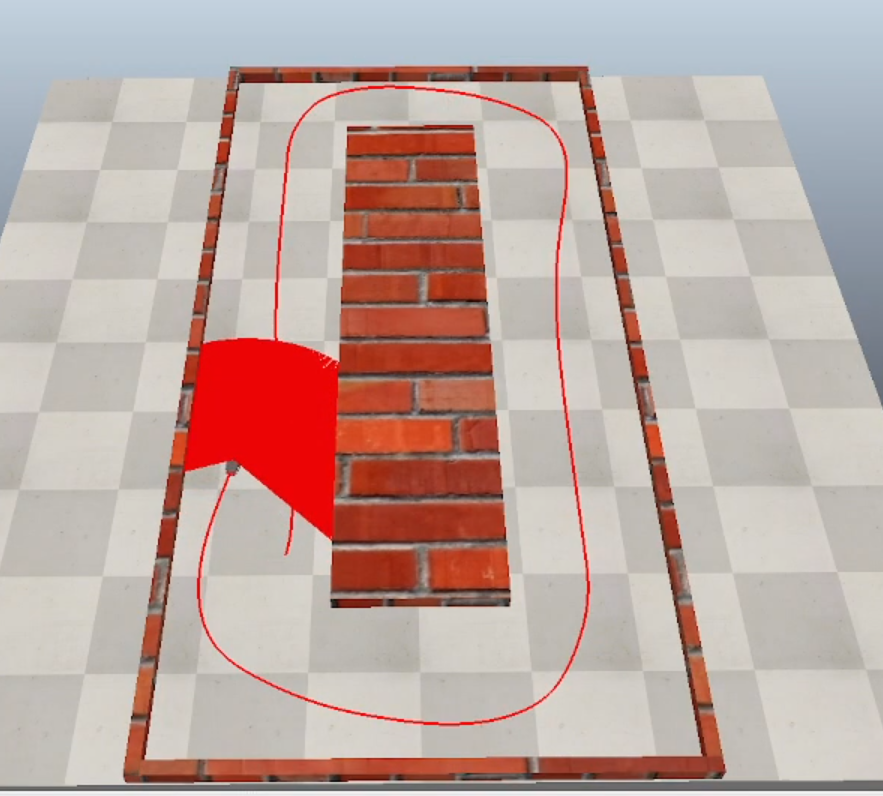
\includegraphics[width=0.85\linewidth]{coppelia_resultado.png}
  \caption{Resultado de la navegaci\'{o}n con estimaci\'{o}n de paredes en \coppelia{}. Se observa el robot \pioneer{} siguiendo el pasillo de forma centrada.}
  \label{fig:coppelia}
\end{figure}


% =====================================================================
%  5. DISCUSIÓN
% =====================================================================
\section{Discusi\'{o}n}

\subsection{Problemas encontrados y soluciones}

\paragraph{Problema 1: puntos de esquina contaminan la regresi\'{o}n.}
Con rangos angulares amplios ($30^\circ$--$150^\circ$) los puntos de las esquinas del pasillo sesgan la recta ajustada, produciendo oscilaciones en la orientaci\'{o}n estimada. \textbf{Soluci\'{o}n}: reducir los rangos a $60^\circ$--$120^\circ$ (pared izquierda) y $-120^\circ$--$-60^\circ$ (pared derecha), limitando la regresi\'{o}n a los puntos que realmente pertenecen a la pared lateral.

\paragraph{Problema 2: divisi\'{o}n por cero en paredes verticales.}
Cuando la pared es aproximadamente perpendicular al eje $x$ del robot, el denominador de la regresi\'{o}n tiende a cero. \textbf{Soluci\'{o}n}: si $|n\sum x_i^2 - (\sum x_i)^2| < 10^{-9}$, se asigna $m = 0$ y $b = \bar{y}$, lo que equivale a modelar la pared como horizontal (caso degenerado seguro).

\paragraph{Problema 3: p\'{e}rdida de pared en curvas.}
Al no implementar un modo de curva dedicado, cuando el robot entra en una curva pierde visibilidad de una pared y el control se detiene. \textbf{Soluci\'{o}n parcial}: la cl\'{a}usula de guarda (\texttt{isfinite(b\_left) \&\& isfinite(b\_right)}) evita comandos err\'{a}ticos. La soluci\'{o}n completa requerir\'{i}a integrar el modo curva de Lab-MR1-II.

\subsection{Limitaciones}
\begin{itemize}[leftmargin=2em]
  \item \textbf{No negocia curvas}: el robot se detiene al perder una pared. Integrar el modo curva de la pr\'{a}ctica anterior resolver\'{i}a este problema.
  \item El modelo lineal \textbf{asume paredes rectas}. En pasillos con paredes curvas la regresi\'{o}n pierde precisi\'{o}n.
  \item Con pocos puntos v\'{a}lidos ($n < 2$), la funci\'{o}n devuelve $b = \infty$ y el robot se detiene innecesariamente. Un umbral m\'{a}s sofisticado o un modelo de respaldo mejorar\'{i}an la disponibilidad.
  \item No se utiliza la pendiente $m$ para anticipar curvas: una pendiente creciente de la pared podr\'{i}a indicar la proximidad de un giro.
\end{itemize}


% =====================================================================
%  6. CONCLUSIONES
% =====================================================================
\section{Conclusiones}
Se ha implementado un controlador de seguimiento de pasillo que sustituye las lecturas puntuales del l\'{a}ser por un \textbf{modelo geom\'{e}trico de paredes} obtenido por regresi\'{o}n lineal. Las mejoras respecto a Lab-MR1-II son:

\begin{enumerate}[leftmargin=2em]
  \item \textbf{Mayor robustez al ruido}: la regresi\'{o}n integra decenas de puntos l\'{a}ser por pared, frente a las ventanas de $\pm 1^\circ$ de la versi\'{o}n anterior.
  \item \textbf{Estimaci\'{o}n directa de orientaci\'{o}n}: la pendiente $m$ de cada pared proporciona la orientaci\'{o}n relativa del robot sin heur\'{i}sticas adicionales.
  \item \textbf{Punto objetivo calculado anal\'{i}ticamente}: $y_\text{goal}$ se obtiene evaluando las rectas de ambas paredes en $x = L$, lo que centra el robot de forma natural.
  \item \textbf{Mayor velocidad de crucero}: la estabilidad del estimador permite operar a \SI{0.50}{\meter\per\second} frente a \SI{0.25}{\meter\per\second}.
\end{enumerate}

La limitaci\'{o}n principal es la ausencia de un modo de curva, que impide la navegaci\'{o}n completa del pasillo. Como trabajo futuro se propone combinar este estimador con el modo curva de Lab-MR1-II, utilizar la pendiente de las paredes como predictor de curvas, y explorar modelos no lineales para pasillos curvos.

\end{document}
